\documentclass[a4paper,12pt]{report}

\usepackage[utf8]{inputenc}
\usepackage{fontenc}
\usepackage{graphicx}

% Remove option to use English naming
\usepackage[italian]{cleveref}

% Questo commentalo se vuoi scrivere in inglese.
\usepackage[italian]{babel}

\title{Smart Experiment\\Second Assignment\\IOT a.a. 2020/21}
 
\author{Ceredi Simone, Conti Alessio}
\date{30/11/2020}


\begin{document}
 
\maketitle

\chapter{Introduzione}
Il progetto vuole modellare un sistema embedded per la valutazione real-time di esperimenti di cinematica.
Questo deve tracciare la posizione, velocità e accelerazione di un corpo che si muove in linea retta. 

Per sviluppare il sistema abbiamo adottato un'architettura a task sincrona, particolarmente adatta allo scopo in quanto la maggior parte degli stati in cui si trova il sistema durante l'esecuzione richiedono una temporizzazione.

\chapter{Diagramma degli stati}
\begin{figure}
\centering{}
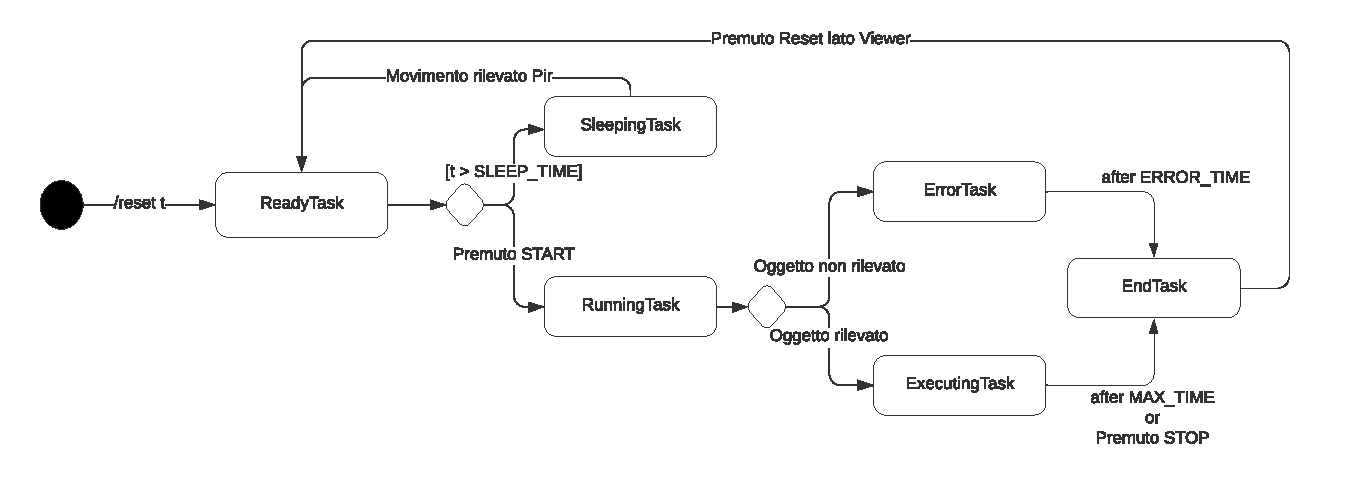
\includegraphics[width=\textwidth]{state_diagram.pdf}
\caption{Schema UML del diagramma degli stati.}
\label{img:state diagram}
\end{figure}
Dall'immagine si può notare la linea di pensiero generale che ci ha guidato alla soluzione dell'esercizio.
Sono stati individuati i task principali (macro-task) che caratterizzano l'esecuzione.
Questi macro-task sono stati individuati pensando al comportamento della macchina nei momenti di interazione con l'utente. 
Talvolta questi possono utilizzare, per meglio gestire il periodo d'esecuzione, task secondari.


\chapter{Descrizione}
Abbiamo abbracciato il paradigma ad oggetti: ogni sensore e attuatore è stato modellato attraverso una classe in c++ con la rispettiva interfaccia, così come ogni task.

A far procedere il sistema è uno scheduler cooperativo implementato tramite una lista. A seconda del proprio periodo di funzionamento questo richiama all'azione i vari task "attivi" per i quali è trascorso un tempo congruo al loro periodo.

Per lo sviluppo abbiamo cercato di mantenere minimale il tempo d'esecuzione di ogni task limitando al massimo il numero di operazioni che esso deve svolgere. Per questo motivo possiamo considerare praticamente nullo il tempo di esecuzione dei task rispetto al periodo con il quale ciclicamente vengono eseguiti. Grazie a questa considerazione semplificativa è stato facile tenere conto del tempo trascorso all'interno dei task stessi. Perciò il tempo trascorso dall'inizio di un task non è altro che il periodo del task moltiplicato per il numero di volte che tale task viene richiamato. Questo piccolo accorgimento ci ha permesso di tenere traccia facilmente delle tempistiche e delle varie sincronizzazioni.
Punto cruciale del progetto è stato scegliere i periodi dei task in modo da non generare perdite di eventi.
Non c'è realmente stato un reale problema di overrun in quanto il sistema è pensato per minimizzare il tempo di esecuzione di ogni task.

\chapter{Task}
\section{ReadyTask}
ReadyTask è il primo stato in cui il sistema entra non appena viene acceso. 
Questo task deve tenere conto del tempo trascorso in quanto deve passare a SleepingTask nel caso in cui non venga effettuato il passaggio a RunningTask in un tempo consono (SLEEP TIME).

\section{SleepingTask}
Tale task modella lo stato di sleep del sistema, più precisamente in power down mode: lo stato di risparmio massimo di energie. 
Per ogni esecuzione viene richiamato soltanto una volta, il suo periodo risulta quindi ininfluente. Ciò è dovuto dal fatto che il sistema finché rimane in sleep non deve operare, ed una volta svegliato grazie al trigger di un pir deve passare la parola al task successivo.

\section{RunningTask}
Questo è un task intermedio per il quale è richiesta una sola iterazione. Si assicura che sia presente un oggetto di fronte al sensore di prossimità e predispone il sistema per il task successivo (ExecutingTask), in caso contrario richiama ErrorTask.

\section{ErrorTask}
ErrorTask sfrutta per il suo funzionamento un task secondario: BlinkTask.

\section{BlinkTask}
Permette il blink di un led che viene passato come parametro al metodo init() del task. Il led lampeggia quindi per un tempo impostato e ad una frequenza ben definita.

\section{ExecutingTask}
ExecutingTask è il task che permette la rilevazione della distanza dell'oggetto ed il calcolo di velocità ed accelerazione, inoltre si occupa dell'invio via seriale dei dati raccolti.

\section{ServoMovementTask}
ServoMovementTask viene utilizzato da ExecutingTask per gestire il movimento del servo e simulare un tachimetro. L’introduzione di tale task si è resa necessaria in quanto il servo non riesce a muoversi di un angolo maggiore di 10° rispetto alla posizione attuale. 

\section{EndExperimentTask}
Tale task viene attivato durante lo stato di Running ed esegue assieme ad ExecutingTask. La sua funzione è terminare l'esecuzione dell'esperimento alla pressione del bottone stop.

\section{EndTask}
Il task finale del sistema, sfrutta il task secondario BlinkTask ed attende l'arrivo di un messaggio sulla seriale per poter riportare il sistema nello stato iniziale di Ready.

\chapter{Java - Smart Exp Viewer}
Il programma in Java che esegue sul calcolatore è stato suddiviso in tre componenti principali: Main, View, DataCollector che possono essere ricondotti ad una semplificazione di MVC.
La classe Main esemplifica il controller, questa riceve i messaggi provenienti dalla seriale e li invia al DataCollector.
La classe DataCollector funge da model. Elabora i dati ricevuti dal Main e li processa per poi passarli alla View.
La classe View si occupa di stampare i dati ricevuti sotto forma grafica in tre diversi grafici. Abbiamo utilizzato la libreria esterna XChart per agevolare tale compito.


\end{document}
